% Options for packages loaded elsewhere
\PassOptionsToPackage{unicode}{hyperref}
\PassOptionsToPackage{hyphens}{url}
%
\documentclass[
]{book}
\usepackage{lmodern}
\usepackage{amsmath}
\usepackage{ifxetex,ifluatex}
\ifnum 0\ifxetex 1\fi\ifluatex 1\fi=0 % if pdftex
  \usepackage[T1]{fontenc}
  \usepackage[utf8]{inputenc}
  \usepackage{textcomp} % provide euro and other symbols
  \usepackage{amssymb}
\else % if luatex or xetex
  \usepackage{unicode-math}
  \defaultfontfeatures{Scale=MatchLowercase}
  \defaultfontfeatures[\rmfamily]{Ligatures=TeX,Scale=1}
\fi
% Use upquote if available, for straight quotes in verbatim environments
\IfFileExists{upquote.sty}{\usepackage{upquote}}{}
\IfFileExists{microtype.sty}{% use microtype if available
  \usepackage[]{microtype}
  \UseMicrotypeSet[protrusion]{basicmath} % disable protrusion for tt fonts
}{}
\makeatletter
\@ifundefined{KOMAClassName}{% if non-KOMA class
  \IfFileExists{parskip.sty}{%
    \usepackage{parskip}
  }{% else
    \setlength{\parindent}{0pt}
    \setlength{\parskip}{6pt plus 2pt minus 1pt}}
}{% if KOMA class
  \KOMAoptions{parskip=half}}
\makeatother
\usepackage{xcolor}
\IfFileExists{xurl.sty}{\usepackage{xurl}}{} % add URL line breaks if available
\IfFileExists{bookmark.sty}{\usepackage{bookmark}}{\usepackage{hyperref}}
\hypersetup{
  pdftitle={Innovation, Developpment et Recherche},
  hidelinks,
  pdfcreator={LaTeX via pandoc}}
\urlstyle{same} % disable monospaced font for URLs
\usepackage{longtable,booktabs}
\usepackage{calc} % for calculating minipage widths
% Correct order of tables after \paragraph or \subparagraph
\usepackage{etoolbox}
\makeatletter
\patchcmd\longtable{\par}{\if@noskipsec\mbox{}\fi\par}{}{}
\makeatother
% Allow footnotes in longtable head/foot
\IfFileExists{footnotehyper.sty}{\usepackage{footnotehyper}}{\usepackage{footnote}}
\makesavenoteenv{longtable}
\usepackage{graphicx}
\makeatletter
\def\maxwidth{\ifdim\Gin@nat@width>\linewidth\linewidth\else\Gin@nat@width\fi}
\def\maxheight{\ifdim\Gin@nat@height>\textheight\textheight\else\Gin@nat@height\fi}
\makeatother
% Scale images if necessary, so that they will not overflow the page
% margins by default, and it is still possible to overwrite the defaults
% using explicit options in \includegraphics[width, height, ...]{}
\setkeys{Gin}{width=\maxwidth,height=\maxheight,keepaspectratio}
% Set default figure placement to htbp
\makeatletter
\def\fps@figure{htbp}
\makeatother
\setlength{\emergencystretch}{3em} % prevent overfull lines
\providecommand{\tightlist}{%
  \setlength{\itemsep}{0pt}\setlength{\parskip}{0pt}}
\setcounter{secnumdepth}{5}
\usepackage{booktabs}
\ifluatex
  \usepackage{selnolig}  % disable illegal ligatures
\fi
\usepackage[]{natbib}
\bibliographystyle{apalike}

\title{Innovation, Developpment et Recherche}
\author{true \and true \and true}
\date{2021-01-13}

\begin{document}
\maketitle

{
\setcounter{tocdepth}{1}
\tableofcontents
}
\hypertarget{objectif}{%
\chapter{Objectif}\label{objectif}}

Ce module a pour objectif de permettre aux étudiants de maîtriser les bases de la recherche scientifique : recherche documentaire ciblée, analyse de documents (essentiellement en langue Anglaise), synthèse sous la forme de la rédaction d'un article, préparer et suivre un protocole expérimental et aussi l'organisation et les modes de financement de la recherche. Le module est organisé en deux volets : méthodologie de recherche et atelier d'écriture

\hypertarget{muxe9thodologie}{%
\chapter{Méthodologie}\label{muxe9thodologie}}

Cet enseignement a pour objectif de permettre aux étudiants de comprendre et d'aborder :

\begin{itemize}
\tightlist
\item
  Comment la connaissance scientifique s'établit, se valide, se valorise et se transfère
\item
  Les méthodologies de recueil et de traitement de l'information (information quantitative, qualitative\ldots) pertinentes au regard des objectifs de recherche,
\item
  Comment poser une question de recherche, sélectionner rapidement des articles pertinents dans les bases de données pour positionner la problématique et la contribution envisagée,
\item
  Comment construire des cas d'étude ou des protocoles expérimentaux au regard de la nature des propositions à valider.
\item
  et plus particulièrement, les théories de l'innovation et les sciences de la conception, ainsi que les revues et conférences spécialisées dans ce domaine.
\end{itemize}

\hypertarget{atelier-duxe9criture-scientifique-et-de-publications}{%
\section{Atelier d'écriture scientifique et de publications}\label{atelier-duxe9criture-scientifique-et-de-publications}}

Cet enseignement a pour objectif de permettre aux étudiants d'améliorer leur pratique de rédaction des rapports et mémoires (notamment pour la rédaction du mémoire de stage).

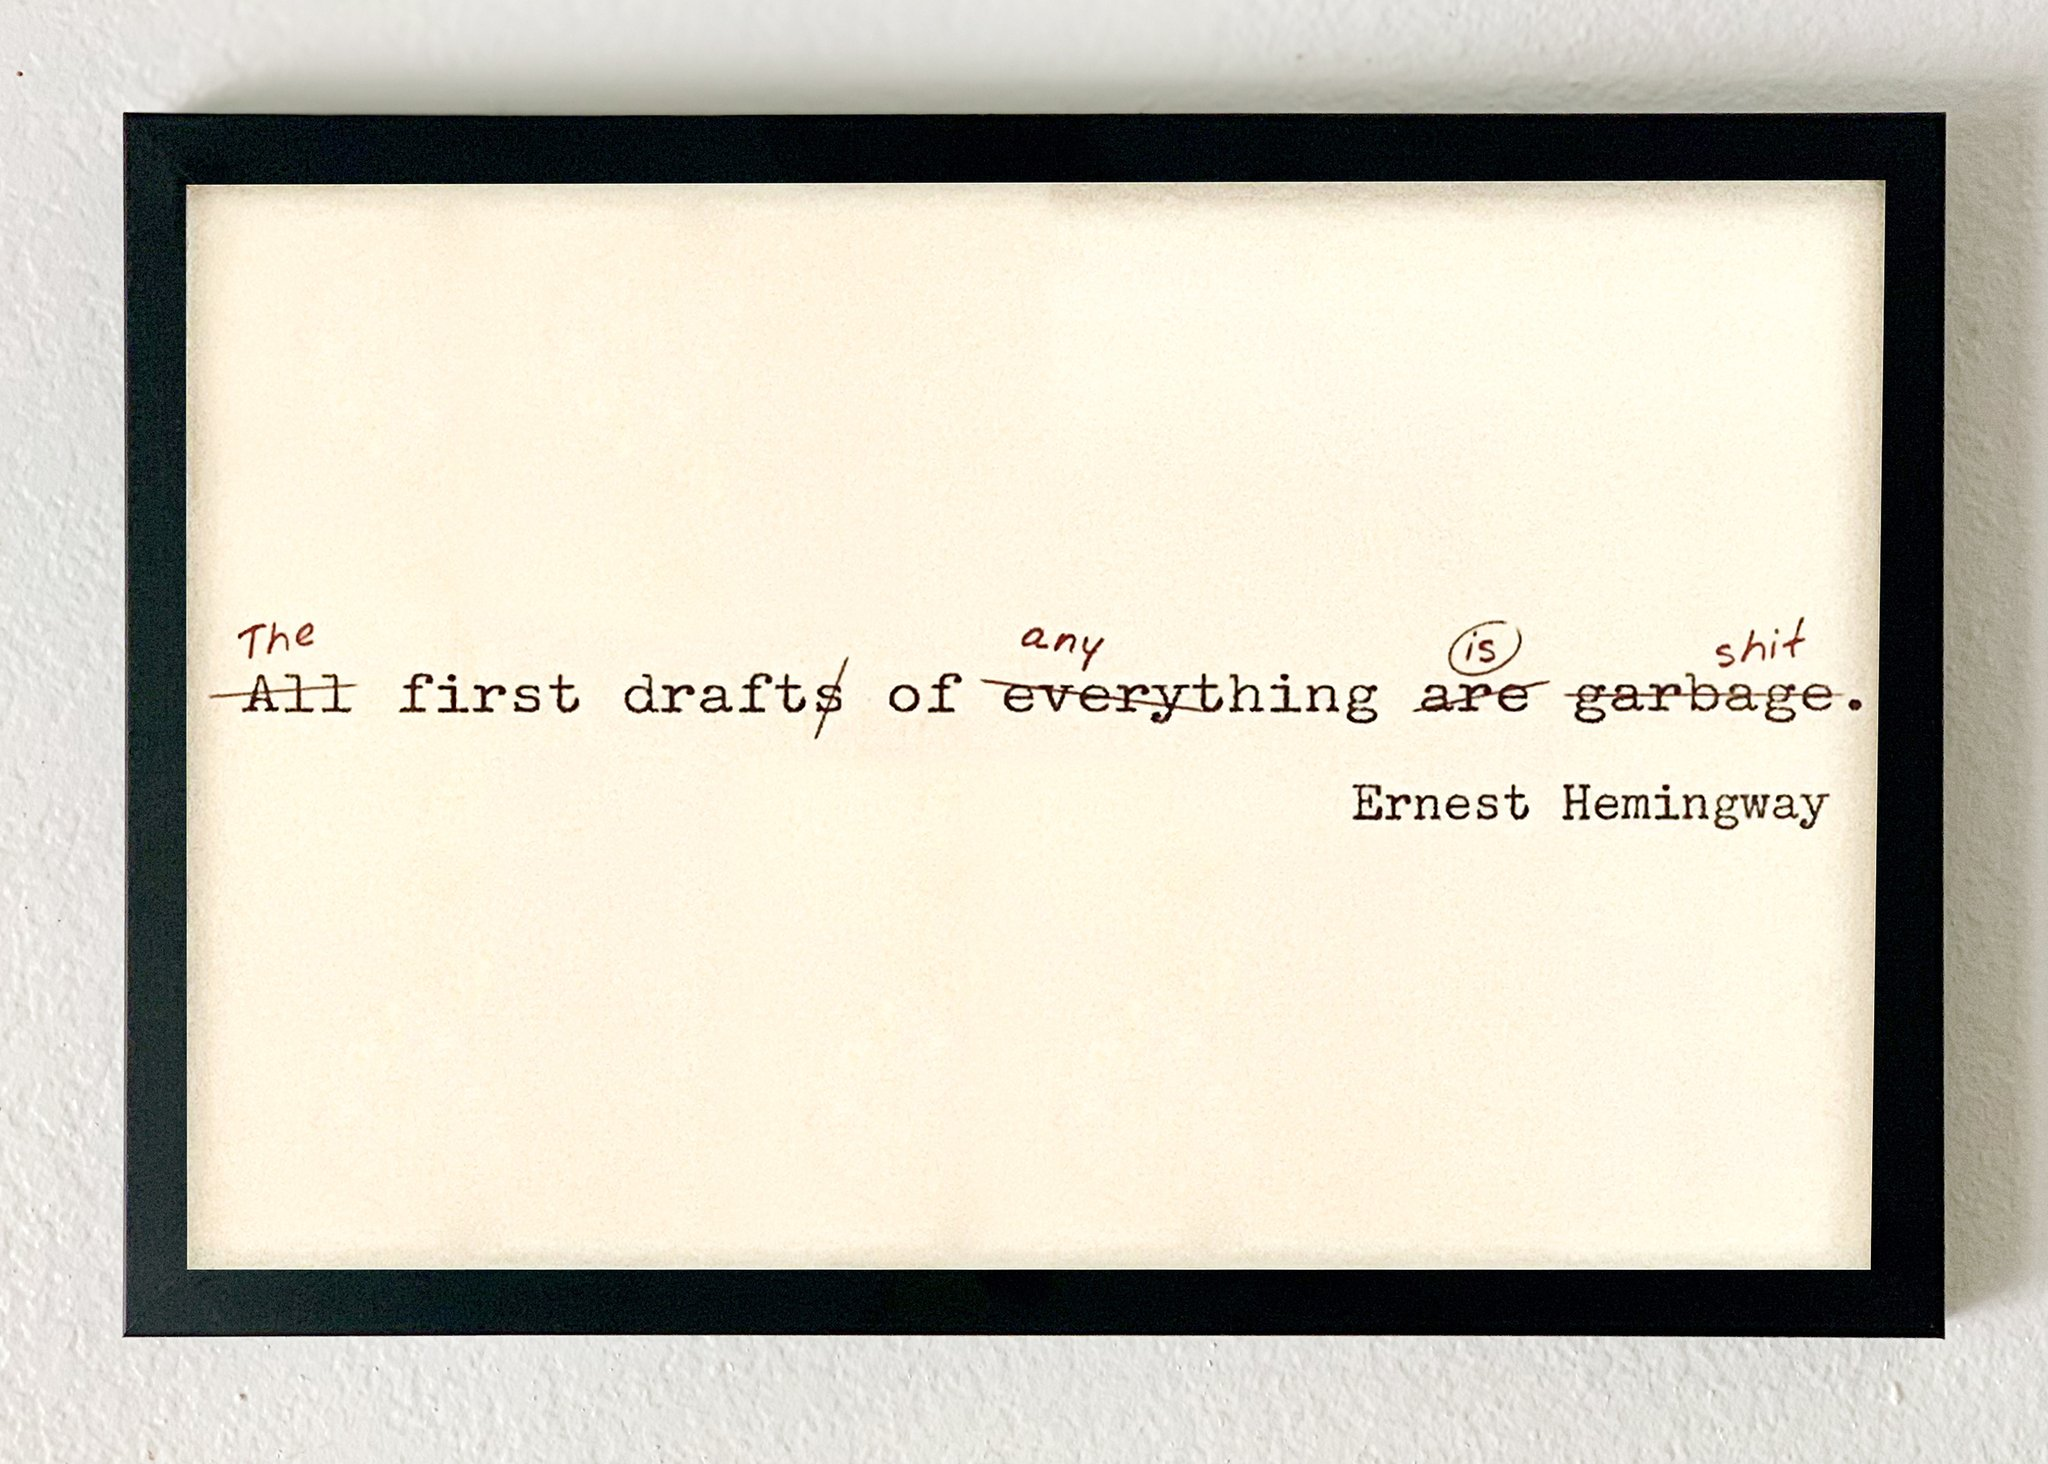
\includegraphics{figures/first-draft.jpg}

\hypertarget{seances}{%
\chapter{Seances}\label{seances}}

Quatre séances d'enseignement aborderont les notions de recherche, veille et état de l'art, protocoles expérimentaux, analyse, traitement et présentation des données.
Chaque séance comporte un travail pratique à rendre à la fin de la séance.

\hypertarget{introduction-cest-quoi-la-recherche}{%
\section{1. Introduction : c'est quoi la recherche ?}\label{introduction-cest-quoi-la-recherche}}

\begin{itemize}
\tightlist
\item
  Conférence recherche laboratoire et entreprise
\item
  Modes de financement de la recherche
\item
  L'État de l'art et VosViewer
\item
  Réalisation d'une exploration d'un domaine scientifique avec VosViewer
\end{itemize}

\hypertarget{concevoir-et-impluxe9menter-un-protocole-expuxe9rimental}{%
\section{2. Concevoir et implémenter un protocole expérimental}\label{concevoir-et-impluxe9menter-un-protocole-expuxe9rimental}}

\begin{itemize}
\tightlist
\item
  Mise en pratique a travers l'évaluation de l'usabilité de sites web
\end{itemize}

\hypertarget{ruxe9daction-des-articles-scientifiques}{%
\section{3. Rédaction des articles scientifiques}\label{ruxe9daction-des-articles-scientifiques}}

\begin{itemize}
\tightlist
\item
  Les outils de gestion bibliographique (Mendeley, Zotero ..)
\item
  Réalisation de fiches de lecture d'articles scientifiques
\item
  Analyse et présentation des données de recherche
\item
  Analyses statistiques
\item
  Rédaction et présentation des résultats
\end{itemize}

\hypertarget{types-de-recherche-applique-thuxe9orique-uxe9tude-de-cas-expuxe9rimentation}{%
\section{4. Types de recherche (applique, théorique, étude de cas, expérimentation)}\label{types-de-recherche-applique-thuxe9orique-uxe9tude-de-cas-expuxe9rimentation}}

\begin{itemize}
\tightlist
\item
  Les articles scientifiques : valorisation des résultats dans la recherche
\item
  Le rapport recherche et l'article état de l'art
\item
  Exemples de rapport recherche
\item
  Validation des sujets pour travail de rédaction
\end{itemize}

\hypertarget{atelier-duxe9criture-scientifique-et-de-publications-1}{%
\section{Atelier d'écriture scientifique et de publications}\label{atelier-duxe9criture-scientifique-et-de-publications-1}}

Rédaction d'un article d'état de l'art sur un sujet donné (de préférence en lien avec le sujet/problématique de la mission de fin d'études)

\hypertarget{modalituxe9s-duxe9valuation}{%
\chapter{Modalités d'évaluation}\label{modalituxe9s-duxe9valuation}}

Chaque séance d'enseignement comporte un composant pratique, les étudiants auront un travail à réaliser et rendre à l'issue de chaque séance : veille scientifique avec VosViewer, mise en pratique d'un protocole expérimental, analyse et présentation des résultats expérimentales.

Pour la partie écriture, le rendu sera fourni sous la forme d'une publication « état de l'art » qui sera évaluée par deux relecteurs de l'équipe pédagogique.

\hypertarget{acknowledgments}{%
\section{Acknowledgments}\label{acknowledgments}}

Ce module est un \emph{Working in Progress} et egalement il est en mode open source.

\hypertarget{introduction}{%
\chapter{Introduction}\label{introduction}}

\hypertarget{presentation}{%
\section{Presentation}\label{presentation}}

Aqui va la presentacion

\hypertarget{introduction-1}{%
\chapter{Introduction}\label{introduction-1}}

\hypertarget{presentation-1}{%
\section{Presentation}\label{presentation-1}}

Aqui va la presentacion

\hypertarget{introduction-2}{%
\chapter{Introduction}\label{introduction-2}}

\hypertarget{presentation-2}{%
\section{Presentation}\label{presentation-2}}

Aqui va la presentacion

\hypertarget{introduction-3}{%
\chapter{Introduction}\label{introduction-3}}

\hypertarget{presentation-3}{%
\section{Presentation}\label{presentation-3}}

Aqui va la presentacion

\hypertarget{references}{%
\chapter{References}\label{references}}

\begin{itemize}
\item
  Chalmers, A. F., \& Biezunski, M. (1990). Qu'est-ce que la science ? : récents développements en philosophie des sciences : Popper, Kuhn, Lakatos, Feyerabend. Librairie générale française.
\item
  Sekaran, Bougie. 2016. Research Methods For Business: A Skill Building Approach. Wiley \& sons.
\item
  Sørensen, Flemming, Jan Mattsson, and Jon Sundbo. 2010. Experimental Methods in Innovation Research. Research Policy 39 (3): 313--22.
\end{itemize}

  \bibliography{biblio.bib}

\end{document}
